\section{Objektív és detektor választás}

\subsection{Paraméterek}
\begin{table}[H]
    \centering
    \begin{tabular}{ll}
        \toprule
        \textbf{Megnevezés és jelölés} & \textbf{Érték} \\
        \midrule
        Tárgy látószöge - $\phi$       & $2^\circ$      \\
        Legkisebb méret - $x$          & 0,5 mm         \\
        Tárgytávolság - $s$            & 100 mm         \\
        Szín                           & Monokróm       \\
        Laterális sebesség - $v$       & 1 m/s          \\
        Megvilágítás                   & NIR            \\
        \bottomrule
    \end{tabular}
\end{table}

\subsection{Fókusztávolság}

A választott kamera pixelmérete legyen a gyakori ipari NIR érzékeny Basler kamerák alapján:
\begin{equation}
    px = 5{,}86 \, \mu\text{m}
\end{equation}
A legkisebb méretet biztonságosan több (minimum kettő, mi esetünkben legyen kb. 10) pixelre érdemes leképezni, így $x$ képe a detektoron (hogy megbízható legyen a detektálás):
\begin{equation}
    y' = 10 \cdot px = 58{,}6 \, \mu\text{m} \approx 0{,}0586 \, \text{mm}
\end{equation}
Ebből kiszámolható az ehhez szükséges nagyítás:
\begin{equation}
    N = \frac{y'}{x} = \frac{0{,}0586}{0{,}5} = 0{,}1172 \, [-]
\end{equation}
A képtávolság:
\begin{equation}
    s' = N \cdot s = 0{,}1172 \cdot 100 \, \text{mm} = 11{,}72 \, \text{mm}
\end{equation}
Ebből a fókusztávolság:
\begin{equation}
    f = \frac{1}{\frac{1}{s'} + \frac{1}{s}} = \frac{1}{\frac{1}{11{,}72} + \frac{1}{100}} = 10{,}49 \, \text{mm} \approx 12 \, \text{mm}
\end{equation}

\newpage
\subsection{Kamerarendszer}
Célszerű egy szabványos, $f = 12 \, \text{mm}$ fókusztávolságú ipari objektívet választani. Legyen ez a katalógusból az \href{https://www.edmundoptics.com/f/c-series-fixed-focal-length-lenses/13679/}{\textbf{Edmund Optics 12mm C Series Fixed Focal Length Lens}}. \\
Ehhez választott fényképezőgép egy \href{https://www.baslerweb.com/en/shop/aca1920-155um/}{\textbf{Basler ace acA1920-155um}}.

Ellenőrzés behelyettesítve a 12~mm-es fókusztávolságot:
\begin{equation}
    s' = \frac{1}{\frac{1}{f} - \frac{1}{s}} = \frac{1}{\frac{1}{12} - \frac{1}{100}} = 13{,}636 \, \text{mm}
\end{equation}
A tényleges nagyítás:
\begin{equation}
    N = \frac{s'}{s} = \frac{13{,}636}{100} = 0{,}1364 \, [-]
\end{equation}
A legkisebb méret képe a detektoron:
\begin{equation}
    y' = N \cdot x = 0{,}1364 \cdot 0{,}5 \, \text{mm} = 0{,}0682 \, \text{mm} = 68{,}2 \, \mu\text{m}
\end{equation}
Ebből pixelekre átszámolva:
\begin{equation}
    \frac{68{,}2}{5{,}86} = 11{,}63 \approx 12 \text{ pixel}
\end{equation}
Ami bőven nagyobb, mint a minimálisan elvárt 2 pixel, ezért biztonságosan detektálható.

\subsection{A tárgy képe a detektoron}
A $2^\circ$-os látószögnek megfelelő tárgyméret:
\begin{equation}
    D = 2 \cdot s \cdot \tan\left(\frac{2^\circ}{2}\right) = 2 \cdot 100 \cdot \tan(1^\circ) = 3{,}49 \, \text{mm}
\end{equation}
A hasznos tárgy mérete a detektoron (sávszélessége):
\begin{equation}
    D' = D \cdot N = 3{,}49 \cdot 0{,}1364 = 0{,}476 \, \text{mm}
\end{equation}
A kamera érzékelőjének fizikai mérete (1920x1200): $11{,}25 \times 7{,}03 \, \text{mm}$.
Látható, hogy az érzékelő jóval nagyobb területet lát, mint a tárgyhoz szükséges $2^\circ$-os FOV mérete, azaz kényelmesen a látótérbe fér.

\newpage
\section{Adatátviteli sebesség}
A tárgy $v = 1 \, \text{m/s}$ sebességgel halad. Az érzékelőn a kép sebessége:
\begin{equation}
    v' = v \cdot N = 1000 \, \text{mm/s} \cdot 0{,}1364 = 136{,}4 \, \text{mm/s}
\end{equation}
Az az időtartam, ameddig a szenzor hosszabbik oldalán (11,25 mm) tartózkodik a tárgy képe:
\begin{equation}
    t = \frac{11{,}25}{136{,}4} = 0{,}0825 \, \text{s} = 82{,}5 \, \text{ms}
\end{equation}
Hogy min. 3 képet rögzítsünk a tárgyról amíg az átér a felvételi területen, a szükséges sebesség:
\begin{equation}
    \text{FPS} \approx \frac{3}{0{,}0825} \approx 37 \text{ FPS}
\end{equation}
A 37 FPS messze alatta van a kamera 164 FPS-es maximális teljesítményének. \\
Adatátviteli sebesség tesztelése USB 3.0 vagy GigE csatlakozón keresztül:
\begin{equation}
    1920 \cdot 1200 \cdot 12 \, \text{bit} \cdot 37 \, \text{FPS} \approx 1023 \, \text{Mb/s} \approx 1 \, \text{Gb/s}
\end{equation}
Ez az USB 3.0 (5 Gbps) kábel-kapacitásnak kényelmesen megfelel. Az optimális expozíció pedig $t_{exp} < 1 \, \text{ms}$ ahhoz, hogy a mozgás-elmosódás elfogadható tartományon belül maradjon a $136{,}4 \, \text{mm/s}$ képsebesség mellett.

\newpage
\section{Dokumentáció}

\begin{figure}[!htb]
    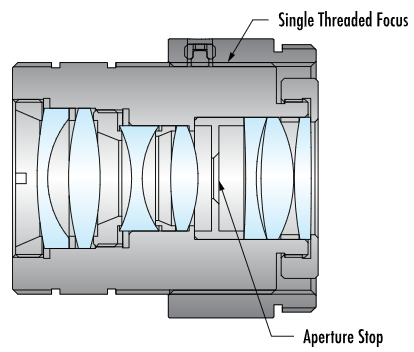
\includegraphics[width=\linewidth]{res/imgs/lens.png}
    \caption{Lencsefoglalás}
\end{figure}
\newpage
\begin{figure}[!htb]
    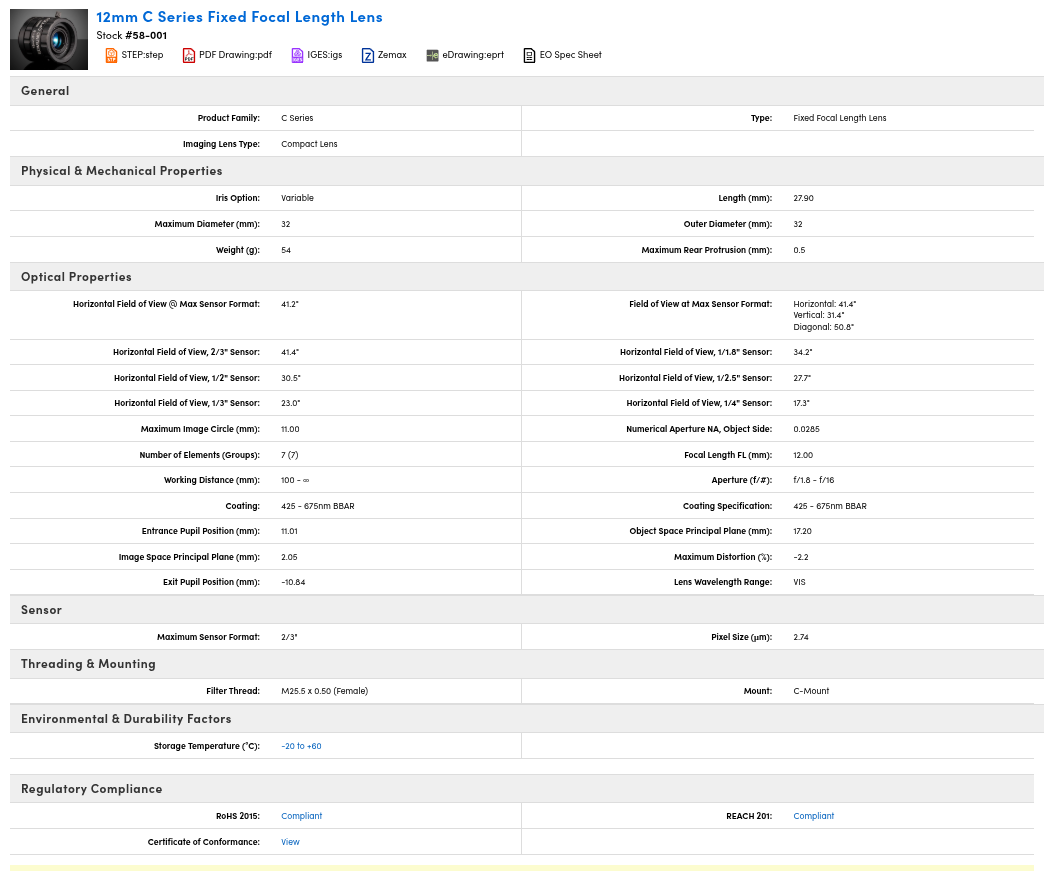
\includegraphics[width=\linewidth]{res/imgs/objective.png}
    \caption{Objektív adatok}
\end{figure}
\newpage
\begin{figure}[!htb]
    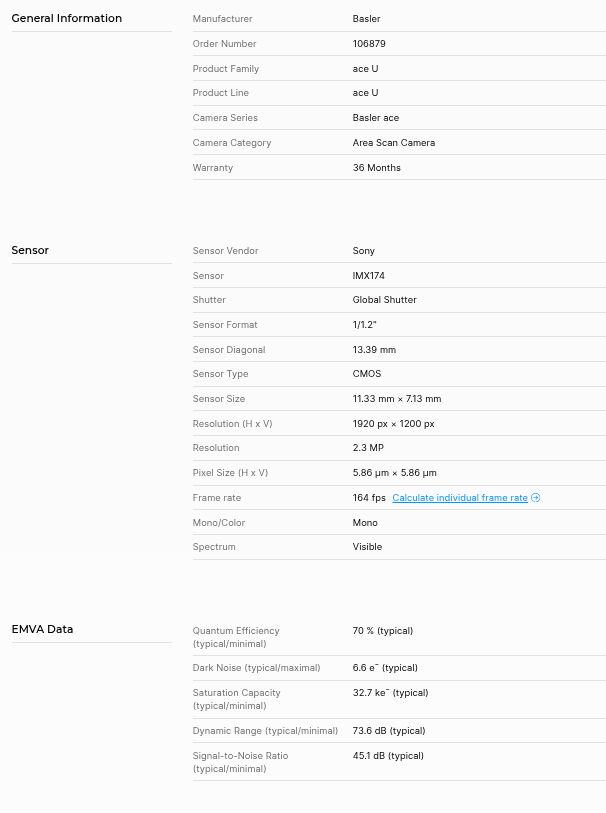
\includegraphics[width=\linewidth]{res/imgs/camera.png}
    \caption{Kamera adatok}
\end{figure}

\newpage
\begin{figure}[H]
    \centering
    \resizebox{\linewidth}{!}{
        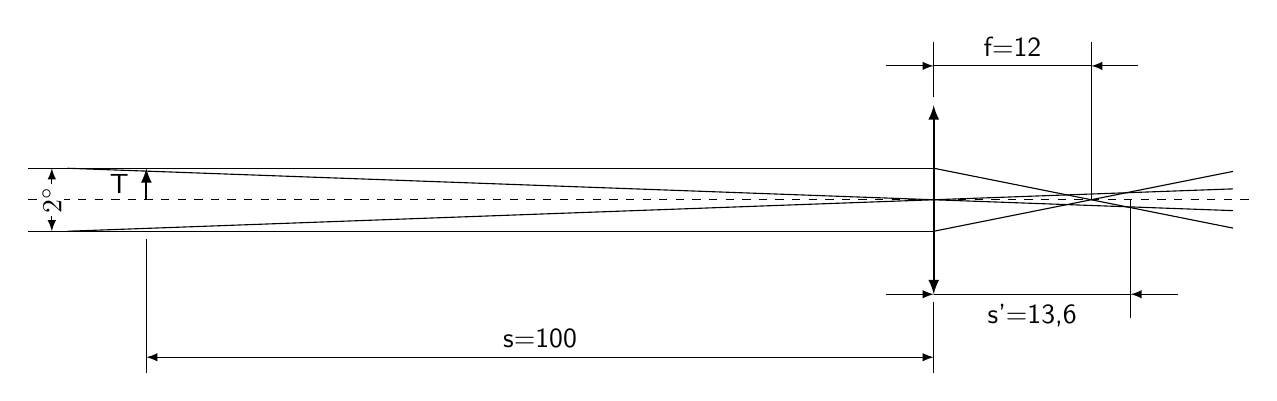
\begin{tikzpicture}[font=\sffamily, >=latex]
            % Optical axis
            \draw[dashed, thin] (-11.5, 0) -- (4, 0);

            % Rays
            % Top parallel ray
            \draw (-11, 0.4) -- (0, 0.4);
            % Top ray bent through focal point
            \draw (0, 0.4) -- (2, 0) -- (3.8, -0.36);
            % Top center ray
            \draw (-11, 0.4) -- (0, 0) -- (3.8, -0.138);

            % Bottom parallel ray
            \draw (-11, -0.4) -- (0, -0.4);
            % Bottom ray bent through focal point
            \draw (0, -0.4) -- (2, 0) -- (3.8, 0.36);
            % Bottom center ray
            \draw (-11, -0.4) -- (0, 0) -- (3.8, 0.138);

            % Lens
            \draw[<->, thick] (0, -1.2) -- (0, 1.2);

            % Object T
            \draw[-latex, thick] (-10, 0) -- (-10, 0.4);
            \node[left] at (-10.1, 0.2) {T};

            % Dimensions
            % 2° FOV
            \draw[very thin] (-11, 0.4) -- (-11.5, 0.4);
            \draw[very thin] (-11, -0.4) -- (-11.5, -0.4);
            \draw[<->] (-11.2, -0.4) -- (-11.2, 0.4) node[midway, fill=white, inner sep=1pt, rotate=90] {$2^\circ$};

            % s = 100
            \draw[very thin] (-10, -0.5) -- (-10, -2.2);
            \draw[very thin] (0, -1.3) -- (0, -2.2);
            \draw[<->] (-10, -2) -- (0, -2) node[midway, above] {s=100};

            % f = 12
            \draw[very thin] (0, 1.3) -- (0, 2);
            \draw[very thin] (2, 0) -- (2, 2);
            \draw (0, 1.7) -- (2, 1.7) node[midway, above] {f=12};
            \draw[<-] (0, 1.7) -- (-0.6, 1.7);
            \draw[<-] (2, 1.7) -- (2.6, 1.7);

            % s' = 13.6
            \draw[very thin] (2.5, 0) -- (2.5, -1.5);
            \draw (0, -1.2) -- (2.5, -1.2) node[midway, below] {s'=13,6};
            \draw[<-] (0, -1.2) -- (-0.6, -1.2);
            \draw[<-] (2.5, -1.2) -- (3.1, -1.2);

        \end{tikzpicture}
    }
    \caption{Optikai sugármenet}
\end{figure}

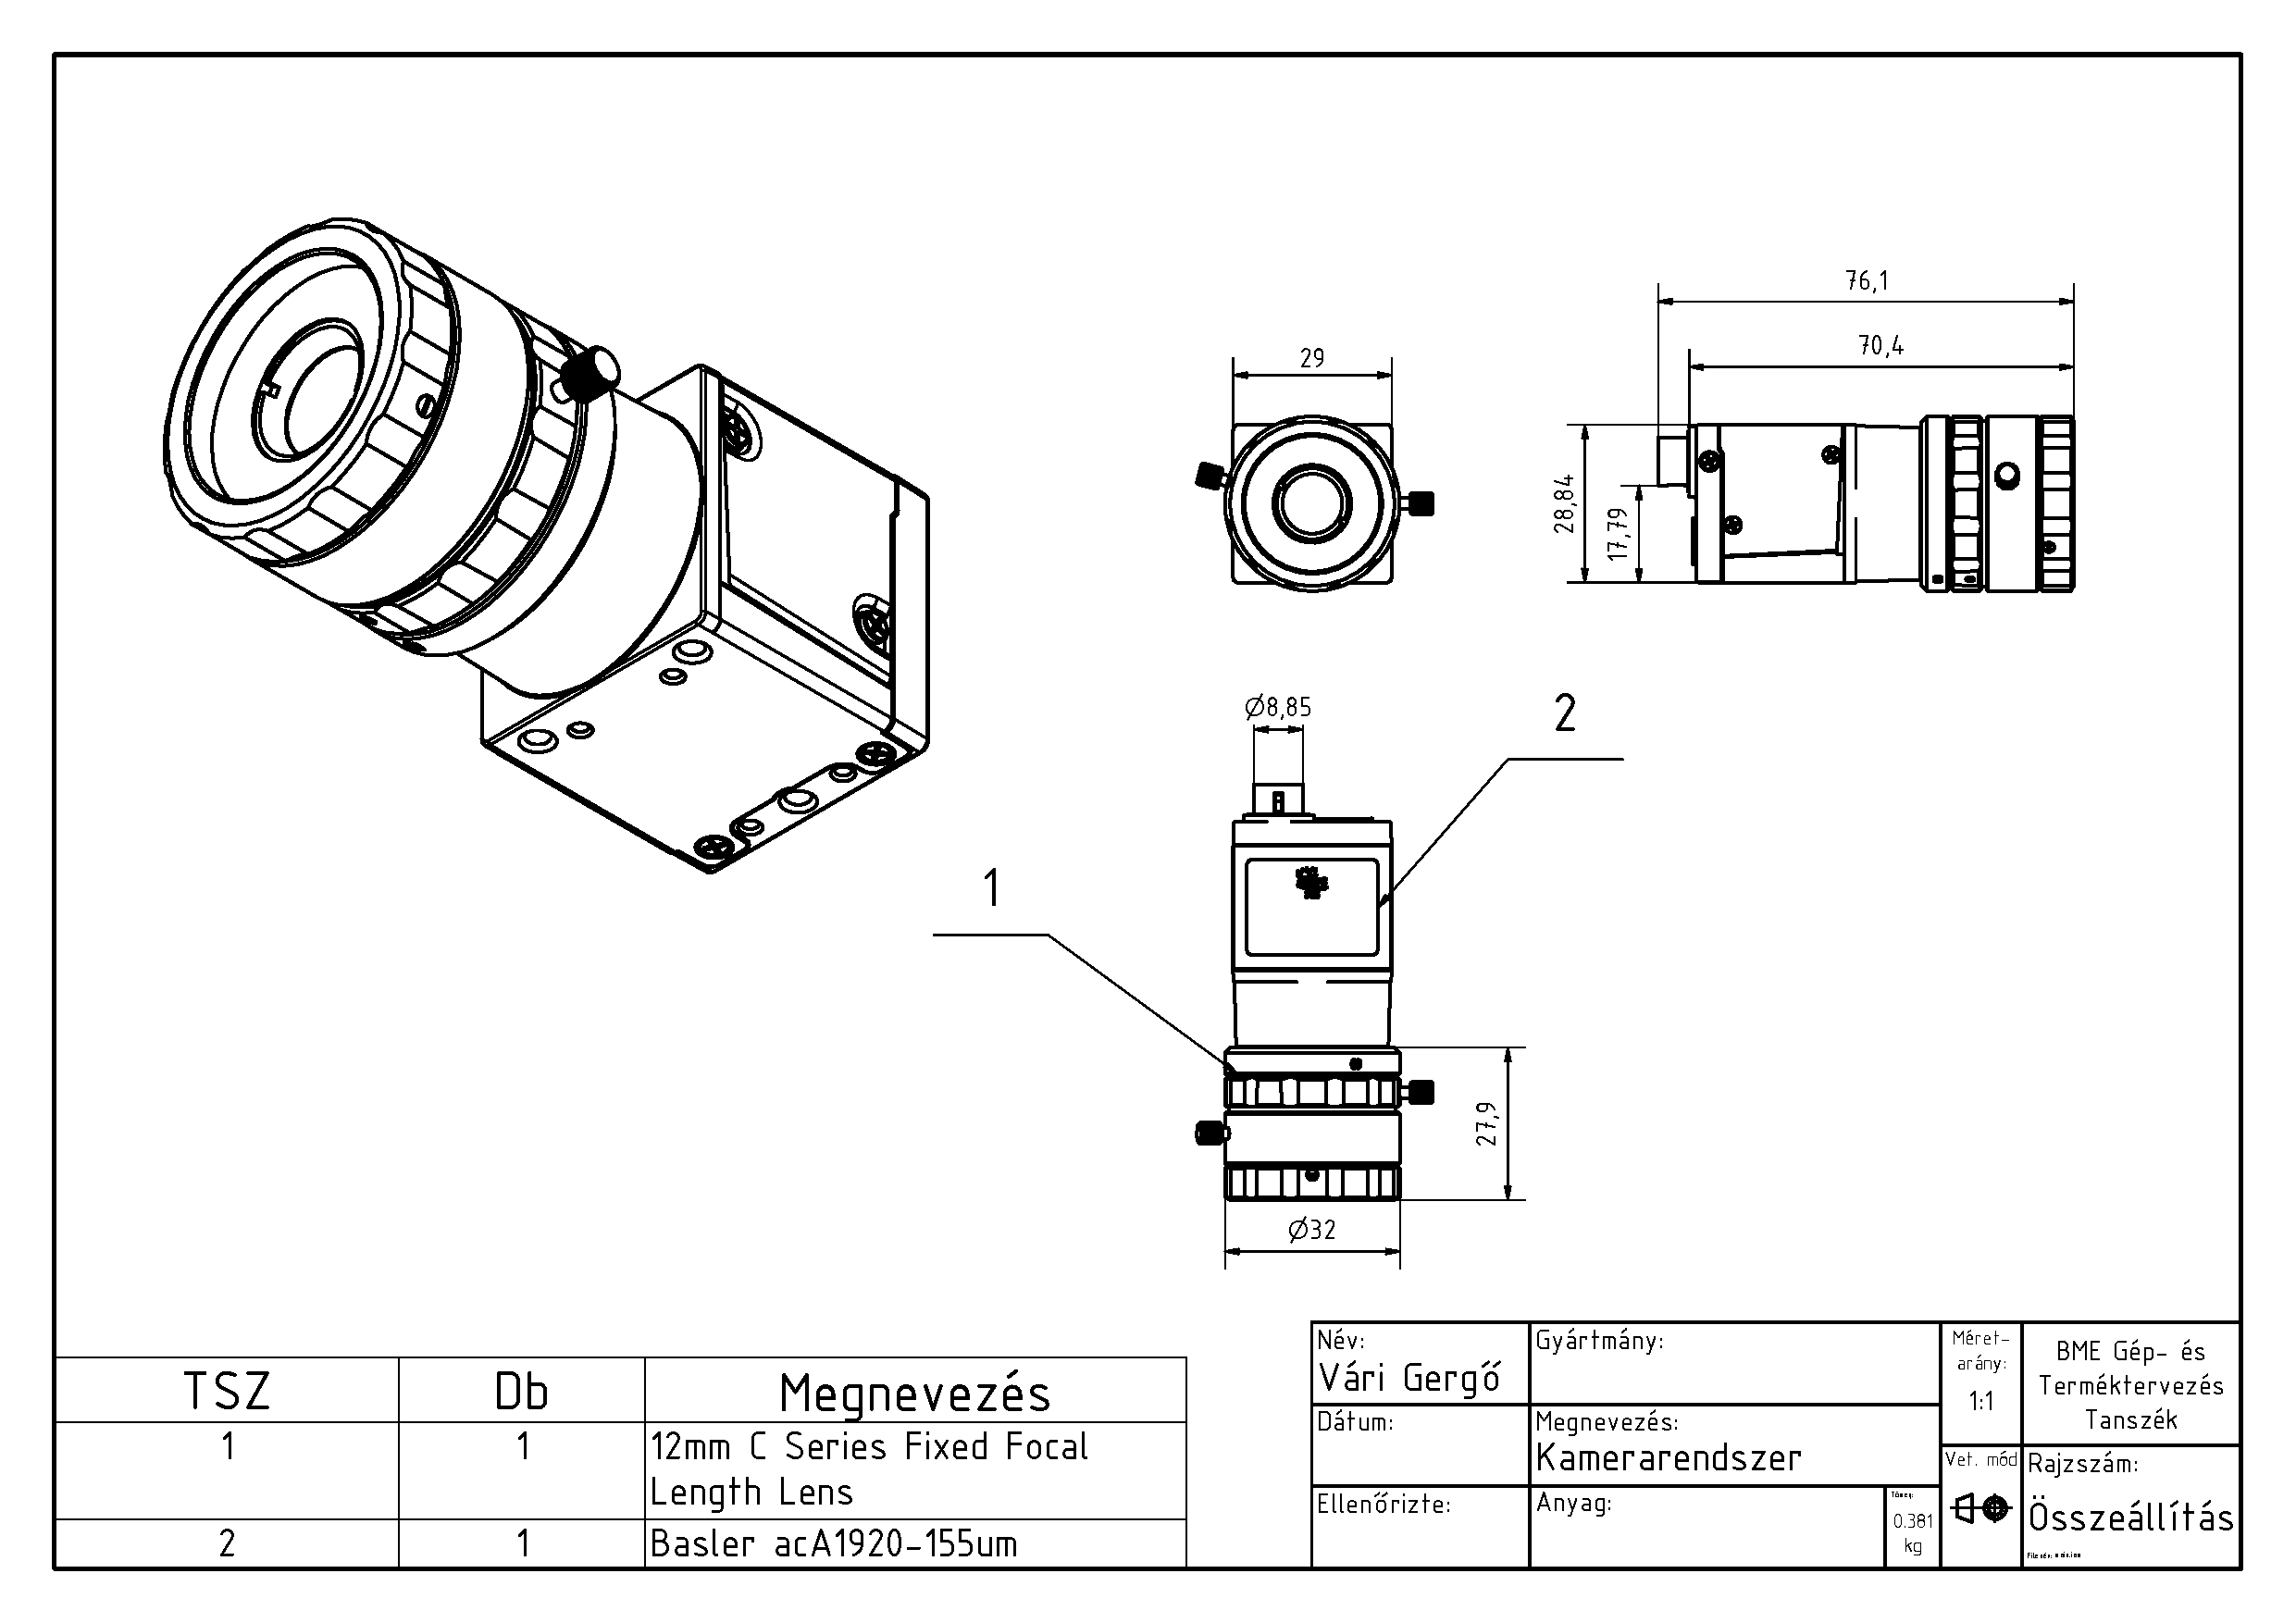
\includepdf{res/drawing.pdf}

\section{Gyakorlati felhasználás}
Az $1 \, \text{m/s}$ laterális sebesség jellemzően egy viszonylag gyors gyártósori futószalag sebességét jelenti. A monokróm, NIR (közeli infravörös) megvilágítást tipikusan olyan gépilátás feladatoknál alkalmazzák, ahol le kell szűrni a környezeti vagy felületi zavaró tényezőket, esetleg be kell látni féligáttetsző csomagolóanyagok felszíne alá (pl. tartalom ellenőrzése teli flakonoknál sötét és átlátszó műanyagok alatt).

Példa: \textbf{Sötét flakonokon gyártási sorja ellenőrzése és minőségbiztosítása} (pl. sorja, mérethibák 0,5 mm pontossággal) alkalmas a rendszer nagy sebesség mellett egy futószalag széléről, zavaró fények beszűrődése nélkül.